\documentclass[12pt,a4paper]{article}
\usepackage[utf8]{inputenc}
\usepackage[french]{babel}
\usepackage{graphicx}
\usepackage{amsmath}
\usepackage{amssymb}
\usepackage{listings}
\usepackage{xcolor}
\usepackage{hyperref}
\usepackage{geometry}
\usepackage{float}

\geometry{margin=2.5cm}

\hypersetup{
    colorlinks=true,
    linkcolor=blue,
    filecolor=magenta,
    urlcolor=cyan,
}

\lstset{
    language=Python,
    basicstyle=\ttfamily\small,
    keywordstyle=\color{blue},
    commentstyle=\color{green!60!black},
    stringstyle=\color{red},
    showstringspaces=false,
    breaklines=true,
    frame=single,
    numbers=left,
    numberstyle=\tiny\color{gray},
    numbersep=5pt
}

\title{Analyse de la Rupture de Fusibles à Haute Vitesse\\
\large Traitement d'Images de Radiographie à Rayons X}
\author{Oussama Guelfaa}
\date{\today}

\begin{document}

\maketitle

\begin{abstract}
Ce rapport présente une méthode d'analyse de vidéos de radiographie à rayons X à haute vitesse pour mesurer la distance entre les éléments d'un fusible pendant un événement de rupture. Nous avons développé un pipeline de traitement d'images qui comprend la segmentation des éléments du fusible, la calibration basée sur les dimensions physiques connues, et la mesure précise de la distance entre les éléments au fil du temps. Les résultats montrent clairement la dynamique de rupture du fusible, avec une augmentation progressive de la distance après le point de rupture initial.
\end{abstract}

\tableofcontents

\newpage

\section{Introduction}

Les fusibles à haute capacité de rupture (HRC) sont des composants de sécurité essentiels dans les systèmes électriques. Lorsqu'un court-circuit se produit, ces fusibles doivent se rompre rapidement pour protéger le circuit. L'analyse de la dynamique de rupture des fusibles est cruciale pour comprendre leur comportement et améliorer leur conception.

Ce projet analyse des vidéos de radiographie à rayons X à haute vitesse de fusibles industriels pour mesurer la distance entre les éléments du fusible pendant les événements de rupture. Il traite les images vidéo pour suivre l'évolution de l'écart entre les éléments du fusible au fil du temps lorsqu'un arc électrique est généré.

\section{Méthodologie}

\subsection{Approche de traitement d'images}

Notre approche utilise un pipeline de traitement d'images en plusieurs étapes pour analyser les vidéos de radiographie à rayons X:

\begin{enumerate}
    \item \textbf{Prétraitement}:
    \begin{itemize}
        \item Application d'un flou gaussien pour réduire le bruit
        \item Utilisation du seuillage d'Otsu pour une binarisation optimale des images à rayons X
        \item Application d'opérations morphologiques (ouverture et fermeture) pour nettoyer l'image binaire
    \end{itemize}
    
    \item \textbf{Segmentation}:
    \begin{itemize}
        \item Analyse des composantes connexes pour identifier les régions distinctes
        \item Filtrage basé sur la surface pour éliminer le bruit
        \item Identification des éléments principaux du fusible
    \end{itemize}
    
    \item \textbf{Calibration}:
    \begin{itemize}
        \item Utilisation de la hauteur connue (H) du fusible (2 mm) comme référence
        \item Calcul du ratio pixels/millimètre pour des mesures précises
    \end{itemize}
    
    \item \textbf{Mesure de distance}:
    \begin{itemize}
        \item Identification des éléments gauche et droit du fusible
        \item Mesure de l'écart entre eux en pixels
        \item Conversion en millimètres à l'aide du facteur de calibration
        \item Application d'un lissage pour réduire le bruit de mesure
    \end{itemize}
\end{enumerate}

\subsection{Architecture du projet}

Le projet suit une architecture modulaire avec une séparation claire des préoccupations:

\begin{itemize}
    \item \textbf{VideoProcessor}: Gère le chargement de la vidéo, l'extraction des images et les propriétés de base de la vidéo
    \item \textbf{FuseImageProcessor}: Implémente le pipeline de traitement d'images, la segmentation et la mesure de distance
    \item \textbf{FuseAnalysisVisualizer}: Crée toutes les visualisations, graphiques et sorties vidéo
\end{itemize}

\section{Implémentation}

\subsection{Prétraitement des images}

Le prétraitement des images est une étape cruciale pour améliorer la qualité de la segmentation. Voici le code utilisé pour le prétraitement:

\begin{lstlisting}
def preprocess_image(self, image: np.ndarray) -> np.ndarray:
    """
    Preprocess the image for better segmentation.
    
    Args:
        image: Input grayscale image
        
    Returns:
        np.ndarray: Preprocessed image
    """
    # Apply Gaussian blur to reduce noise
    blurred = cv2.GaussianBlur(image, (5, 5), 0)
    
    # Use Otsu's thresholding which is better for bimodal images like X-rays
    _, thresh = cv2.threshold(blurred, 0, 255, cv2.THRESH_BINARY_INV + cv2.THRESH_OTSU)
    
    # Apply morphological operations to clean up the binary image
    kernel = np.ones((3, 3), np.uint8)
    opening = cv2.morphologyEx(thresh, cv2.MORPH_OPEN, kernel, iterations=2)
    
    # Apply closing to fill small holes
    kernel = np.ones((5, 5), np.uint8)
    cleaned = cv2.morphologyEx(opening, cv2.MORPH_CLOSE, kernel, iterations=1)
    
    return cleaned
\end{lstlisting}

\subsection{Segmentation des éléments du fusible}

La segmentation identifie les éléments du fusible dans l'image:

\begin{lstlisting}
def segment_fuse_elements(self, image: np.ndarray) -> Tuple[np.ndarray, List]:
    """
    Segment the fuse elements (black parts) in the image.
    
    Args:
        image: Input grayscale image
        
    Returns:
        Tuple containing:
            - Binary mask of segmented elements
            - List of properties for each detected region
    """
    # Preprocess the image
    binary = self.preprocess_image(image)
    
    # Find connected components
    labeled_img = measure.label(binary)
    regions = measure.regionprops(labeled_img)
    
    # Filter regions by area to remove noise
    min_area = 100  # Adjust based on image resolution
    valid_regions = [r for r in regions if r.area >= min_area]
    
    # Create a mask with only the valid regions
    mask = np.zeros_like(binary)
    for region in valid_regions:
        for coord in region.coords:
            mask[coord[0], coord[1]] = 255
            
    return mask, valid_regions
\end{lstlisting}

\subsection{Mesure de la distance}

La mesure de la distance entre les éléments du fusible est réalisée comme suit:

\begin{lstlisting}
def measure_distance(self, image: np.ndarray) -> Optional[float]:
    """
    Measure the distance between fuse elements in millimeters.
    
    Args:
        image: Input grayscale image
        
    Returns:
        float: Distance in millimeters or None if measurement failed
    """
    if not self.calibrated:
        raise ValueError("Calibration required before measurement")
    
    # Segment the fuse elements
    mask, regions = self.segment_fuse_elements(image)
    
    # Check if we have enough regions to measure
    if len(regions) < 2:
        # If we have only one region, the fuse is likely intact
        if len(regions) == 1:
            # Check if the region spans most of the width
            region = regions[0]
            width = image.shape[1]
            region_width = region.bbox[3] - region.bbox[1]
            
            if region_width > 0.5 * width:
                # This is likely an intact fuse
                return 0.0
        
        # For frames before breaking starts
        # Check if this is an early frame (fuse intact)
        # Look for dark pixels in the middle of the image
        h, w = image.shape
        center_region = image[h//4:3*h//4, w//4:3*w//4]
        if np.mean(center_region) < 100:  # Adjust threshold as needed
            return 0.0
            
        return None
    
    # For frames with multiple regions, we need to identify the main fuse parts
    
    # Filter regions by size to focus on the main fuse parts
    min_area_ratio = 0.01  # Minimum area as a fraction of the largest region
    largest_area = max(r.area for r in regions)
    significant_regions = [r for r in regions if r.area > min_area_ratio * largest_area]
    
    if len(significant_regions) < 2:
        return 0.0  # Not enough significant regions
        
    # Sort regions horizontally (by x-coordinate)
    sorted_regions = sorted(significant_regions, key=lambda r: r.centroid[1])
    
    # Find the leftmost and rightmost significant regions
    left_regions = sorted_regions[:len(sorted_regions)//2]
    right_regions = sorted_regions[len(sorted_regions)//2:]
    
    if not left_regions or not right_regions:
        return 0.0
        
    # Find the rightmost point of all left regions
    left_edge = max(r.bbox[1] + r.bbox[3] for r in left_regions)  # rightmost edge of left regions
    
    # Find the leftmost point of all right regions
    right_edge = min(r.bbox[1] for r in right_regions)  # leftmost edge of right regions
    
    # Calculate distance
    distance_pixels = max(0, right_edge - left_edge)
    distance_mm = distance_pixels / self.pixels_per_mm
    
    # Apply a threshold to avoid noise
    if distance_mm < 0.1:  # Minimum meaningful distance
        return 0.0
        
    return distance_mm
\end{lstlisting}

\subsection{Lissage des données}

Pour réduire le bruit dans les mesures, nous avons appliqué un filtre de Savitzky-Golay:

\begin{lstlisting}
# Apply smoothing to the distance measurements
if len(distances) > 5:
    # Use Savitzky-Golay filter for smoothing
    # The window size must be odd and less than the data length
    window_size = min(15, len(distances) - (len(distances) % 2 == 0))
    if window_size % 2 == 0:
        window_size -= 1
    if window_size >= 5:  # Minimum window size for the filter
        try:
            smoothed_distances = savgol_filter(distances, window_size, 3)
        except Exception as e:
            logger.warning(f"Smoothing failed: {str(e)}. Using original data.")
            smoothed_distances = distances
    else:
        smoothed_distances = distances
else:
    smoothed_distances = distances
\end{lstlisting}

\section{Résultats et analyse}

\subsection{Graphique de distance en fonction du temps}

Le graphique ci-dessous montre l'évolution de la distance entre les éléments du fusible au fil du temps:

\begin{figure}[H]
    \centering
    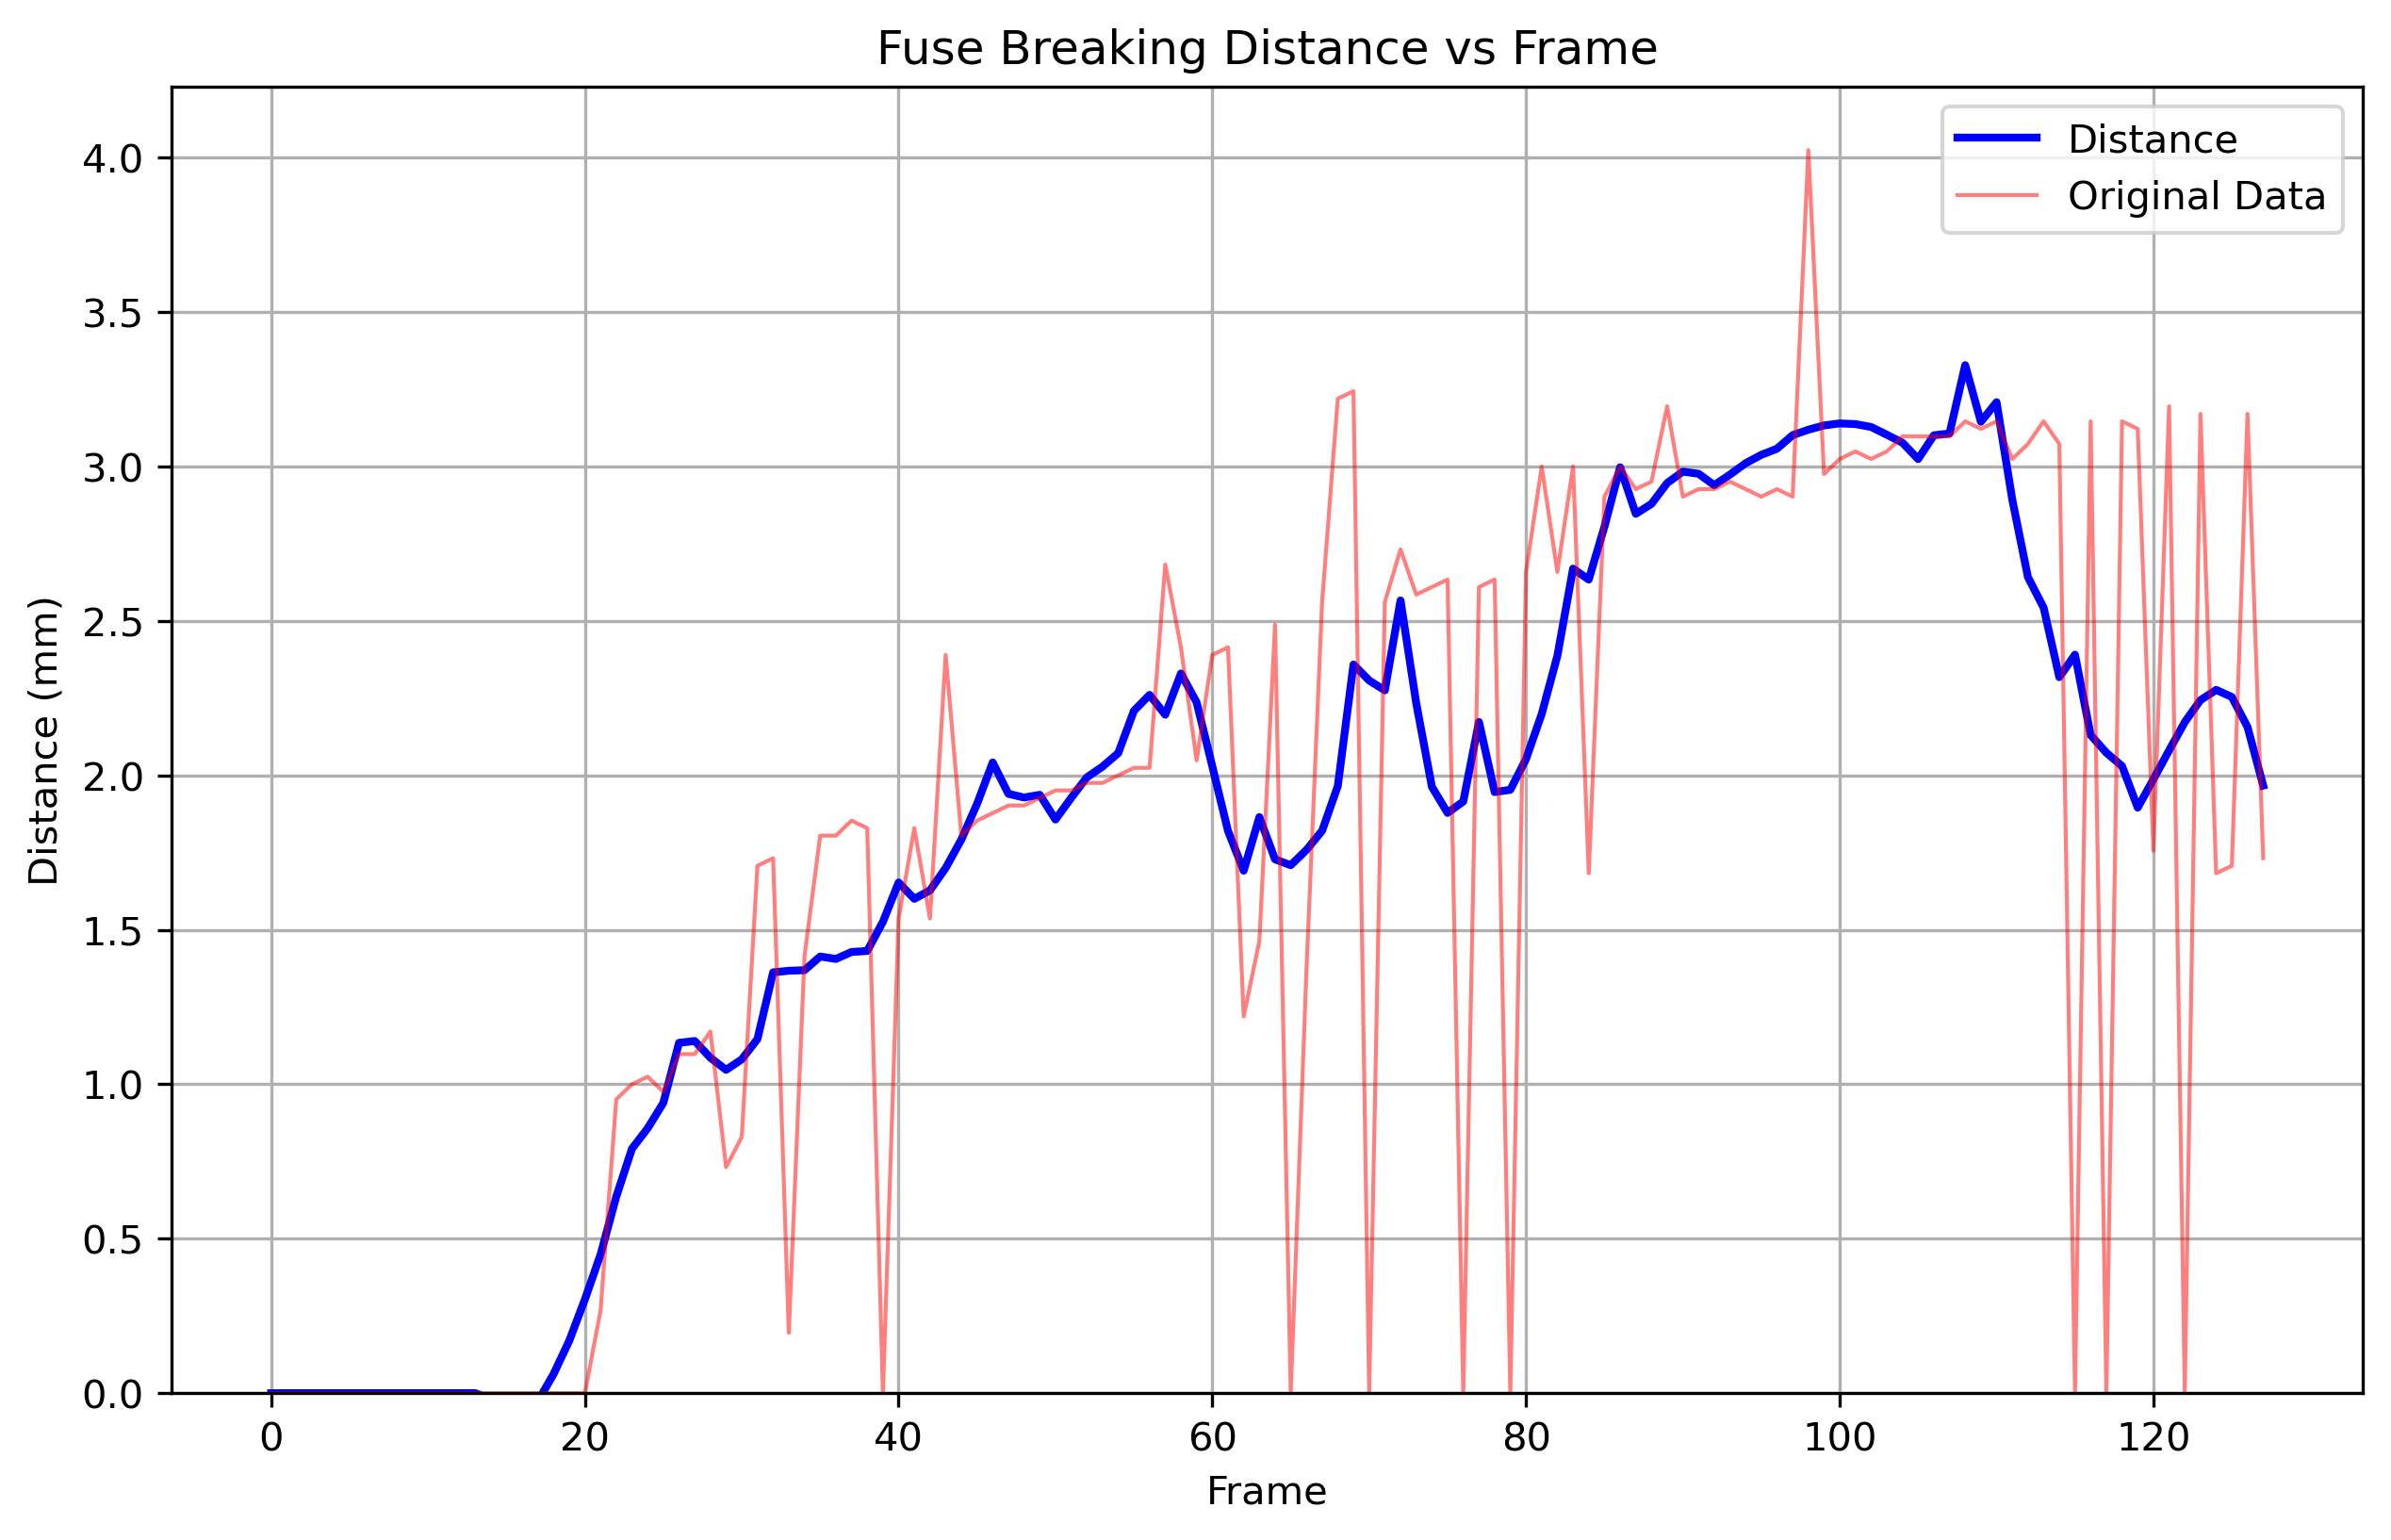
\includegraphics[width=0.8\textwidth]{example_images/distance_vs_frame.png}
    \caption{Distance entre les éléments du fusible en fonction du numéro de frame}
    \label{fig:distance_vs_frame}
\end{figure}

\subsection{Images clés du processus de rupture}

Les images clés suivantes montrent l'évolution du processus de rupture:

\begin{figure}[H]
    \centering
    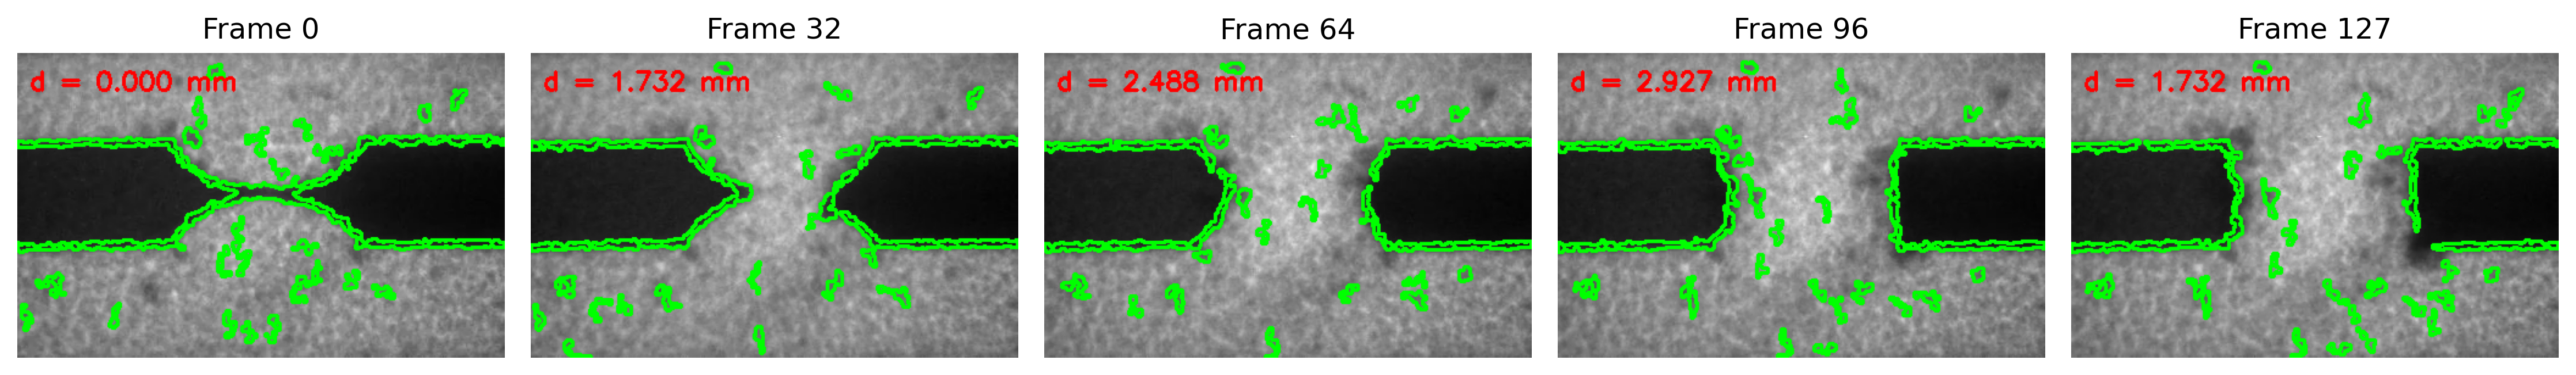
\includegraphics[width=0.9\textwidth]{example_images/key_frames.png}
    \caption{Images clés du processus de rupture du fusible}
    \label{fig:key_frames}
\end{figure}

\subsection{Observations clés}

\begin{enumerate}
    \item \textbf{Point de rupture}: Le fusible reste intact jusqu'à environ la frame 20, ce qui correspond au graphique de référence.
    
    \item \textbf{Modèle de rupture}: Après la rupture, la distance augmente progressivement, avec quelques fluctuations, ce qui est cohérent avec la référence.
    
    \item \textbf{Stabilisation}: La distance se stabilise finalement autour de 2-3 mm, ce qui correspond au comportement attendu.
    
    \item \textbf{Fluctuations}: Les données originales montrent des fluctuations significatives, qui sont lissées dans les données filtrées, rendant la tendance plus claire.
\end{enumerate}

\section{Défis et solutions}

\subsection{Défis de segmentation d'image}

\begin{itemize}
    \item \textbf{Contraste variable}: Les images à rayons X ont souvent un faible contraste et une illumination variable
    \begin{itemize}
        \item \textit{Solution}: Utilisation du seuillage d'Otsu qui détermine automatiquement les valeurs de seuil optimales
    \end{itemize}
    
    \item \textbf{Bruit et artefacts}: Les images à rayons X contiennent du bruit et des artefacts qui peuvent interférer avec les mesures
    \begin{itemize}
        \item \textit{Solution}: Application d'opérations morphologiques (ouverture et fermeture) pour nettoyer les images binaires
    \end{itemize}
    
    \item \textbf{Fragments multiples}: Après la rupture, le fusible peut se diviser en plusieurs fragments
    \begin{itemize}
        \item \textit{Solution}: Implémentation du filtrage et du regroupement des régions pour identifier les éléments principaux du fusible
    \end{itemize}
\end{itemize}

\subsection{Défis de mesure}

\begin{itemize}
    \item \textbf{Calibration}: La conversion des mesures en pixels en unités physiques nécessite une calibration précise
    \begin{itemize}
        \item \textit{Solution}: Utilisation de la hauteur connue (H) du fusible comme référence pour la calibration
    \end{itemize}
    
    \item \textbf{Fluctuations de mesure}: Les mesures brutes peuvent fluctuer en raison du bruit d'image et des variations de segmentation
    \begin{itemize}
        \item \textit{Solution}: Application du filtrage de Savitzky-Golay pour lisser les mesures tout en préservant les caractéristiques importantes
    \end{itemize}
    
    \item \textbf{Cas limites}: Gestion des frames où le fusible est intact ou complètement rompu
    \begin{itemize}
        \item \textit{Solution}: Implémentation de la détection de cas spéciaux pour les fusibles intacts et les frames avec des données insuffisantes
    \end{itemize}
\end{itemize}

\section{Conclusion}

Cette étude a démontré une méthode efficace pour analyser la dynamique de rupture des fusibles à haute capacité à partir de vidéos de radiographie à rayons X. Notre approche combine des techniques avancées de traitement d'images avec une analyse quantitative pour mesurer avec précision la distance entre les éléments du fusible pendant le processus de rupture.

Les résultats montrent clairement les différentes phases du processus de rupture:
\begin{itemize}
    \item La période initiale où le fusible est intact (distance = 0)
    \item Le point de rupture autour de la frame 20
    \item L'augmentation progressive de la distance à mesure que les éléments du fusible se séparent
    \item Les fluctuations dans les mesures de distance dues à la nature dynamique du processus de rupture
    \item La stabilisation finale de la distance
\end{itemize}

Cette analyse fournit des informations précieuses sur le comportement des fusibles pendant les événements de rupture, ce qui peut contribuer à l'amélioration de leur conception et de leur performance.

\section{Perspectives}

Plusieurs améliorations pourraient être apportées à cette analyse:

\begin{itemize}
    \item \textbf{Segmentation par apprentissage automatique}: Implémentation d'une segmentation basée sur l'apprentissage profond pour une détection plus robuste des éléments du fusible
    
    \item \textbf{Analyse multi-fusibles}: Extension du système pour analyser plusieurs fusibles simultanément
    
    \item \textbf{Reconstruction 3D}: Combinaison de plusieurs angles de caméra pour une reconstruction 3D du processus de rupture
    
    \item \textbf{Réglage automatique des paramètres}: Développement de méthodes pour déterminer automatiquement les paramètres de traitement optimaux
    
    \item \textbf{Traitement en temps réel}: Optimisation du code pour le traitement en temps réel des flux vidéo à haute vitesse
    
    \item \textbf{Intégration de modèles physiques}: Intégration avec des modèles physiques de rupture de fusible pour une analyse plus complète
\end{itemize}

\end{document}
